\documentclass[border=10pt]{standalone}
\usepackage{pgfplots}
\pgfplotsset{compat=1.18}
\usepgfplotslibrary{fillbetween}
\begin{document}
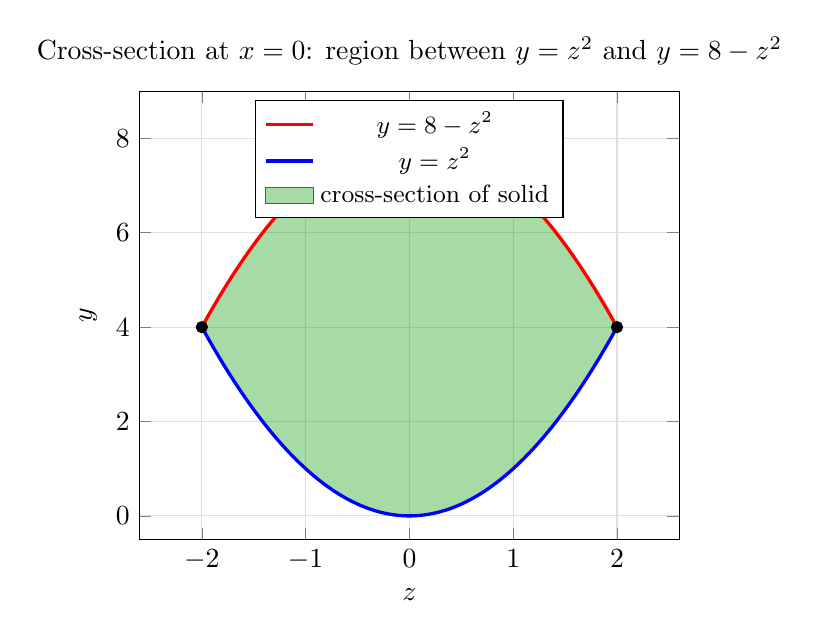
\begin{tikzpicture}
\begin{axis}[
    xlabel={$z$}, ylabel={$y$},
    xmin=-2.6, xmax=2.6, ymin=-0.5, ymax=9,
    domain=-2:2, samples=100,
    grid=major, grid style={gray!25},
    legend style={at={(0.5,0.98)}, anchor=north, font=\small},
    title={Cross-section at $x=0$: region between $y=z^2$ and $y=8-z^2$}
]
% Shaded region between
\addplot[name path=upper, red, very thick] {8-x^2};
\addlegendentry{$y = 8-z^2$}
\addplot[name path=lower, blue, very thick] {x^2};
\addlegendentry{$y = z^2$}
\addplot[green!60!black, fill opacity=0.35] fill between[of=upper and lower];
\addlegendentry{cross-section of solid}
% Intersection points
\addplot[only marks, mark=*, black] coordinates {(-2,4) (2,4)};
\end{axis}
\end{tikzpicture}
\end{document}